\documentclass[xcolor=table]{beamer}

\usepackage[polish]{babel}
\usepackage[utf8]{inputenc}
\usepackage[T1]{fontenc}
\usepackage{listings}
\usepackage{lmodern}
\usepackage{textcomp}


\usetheme[language=polish]%
  {Goddard}

\newcommand{\filepath}{\texttt}
\newcommand{\command}{\texttt}
\newcommand{\email}[1]{\href{mailto:#1}{\texttt{#1}}}
\newcommand{\latexcode}{\texttt}
\newcommand{\parameter}[1]{\textlangle #1\textrangle}


\lstset{basicstyle=\ttfamily,keywordstyle=\color{goddardblue}\bfseries,commentstyle=\color{goddardblue!75}\itshape,columns=flexible}

\rowcolors{1}{goddardblue!50}{goddardblue!30}


\title{Metody rozpoznawania twarzy}
\subtitle{przeglad i porównanie}
\author{Bartłomiej Bułat\\
Tomasz Czarnik\\
Krzysztof Śmiłek\\}


\begin{document}

%==============================
\begin{frame}
  \titlepage
\end{frame}


%==============================
\begin{frame}
  \frametitle{Plan}
  \tableofcontents
\end{frame}


%=============================================================
\section{Wstęp}

\begin{frame}
  \frametitle{Wstęp}
  Rozpoznawanie twarzy to najbardziej naturalny sposób identyfikacji osób. Wraz z rozwojem technologii i mocy obliczeniowej szuka się coraz doskonalszych rozwiązań uskuteczniających to zadanie.\\[\baselineskip]
\uncover <2-> {Przykładowe zastosowania:
\begin{itemize}
\item Fotografia cyfrowa
\item Metody autoryzacji
\item Bezpieczeństwo w strefie publicznej
\item Rozrywka (konsole nowej generacji)
\end{itemize}}
\end{frame}

\subsection{Problem i ogólny algorytm}
\begin{frame}
\frametitle{Problem rozpoznawania twarzy}

Podstawowym problemem w rozpoznawaniu twarzy jest jej właściwa akwizycja. Uzyskanie obrazu z twarzą zwróconą do kamery na jednolitym tle jest nie możliwe w wielu przypadkach zastosowania metody.
\pause

Aby zwalczyć te problemy wykorzystuje się preprocesing lub akwizycje niosącą więcej cech (obrazy termowizyjne lub stereowizyjne).
\pause

Problemem klasyfikacji obiektów jest to, że trudno opisać niezmiennicze cechy w tak zróżnicowanym obiekcie jakim jest twarz.   

\end{frame}

%=============================================================
\section{Na wesoło}
\begin{frame}
  \frametitle{Wykrywanie twarzy na wesoło}

\begin{figure}
 \only<1> {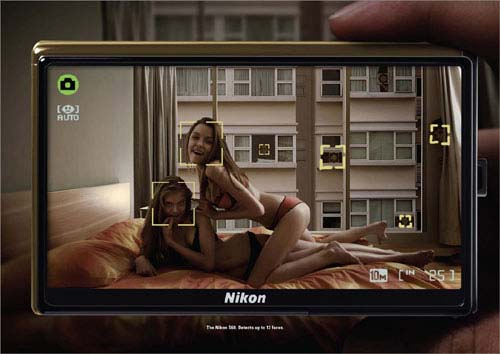
\includegraphics[scale=0.5]{funny.jpg}}
\caption{ Nie-poważny przykład zastosowania detekcji twarzy}
\end{figure}

\end{frame}

%==============================
\begin{frame}
  \frametitle{Ogólny algorytm}

\begin{enumerate}
\item Akwizycja obrazu (uzyskanie obrazu pozwalającego na lokalizacje twarzy) \pause
\item Ekstrakcja cech (opisanie wybranych obiektów) \pause
\item Klasyfikacja (określenie obiektów jako twarz lub nie)
\end{enumerate}
   
\end{frame}


%=============================================================
\section{Metody rozpoznawania twarzy}

%=============================================================
\subsection{Metody geometryczne}
\begin{frame}
  \frametitle{Metody geometryczne}

Jest to jedno z pierwszych, najbardziej intuicyjnych podejść w dziedzinie rozpoznawania twarzy. \\
Twarz charakteryzowana jest przez zbiór wartości kątów, odległości czy też pól wyznaczonych w oparciu \\
o charakterystyczne punkty na obrazie. \\
Badane są między innymi:
\begin{itemize}
\item szerokość/wysokość twarzy
\item szerokość/długość nosa
\item odległości między: linią oczu i linią ust, środkami oczu, najdalszymi/najbliższymi punktami oczu, oczami i nosem
\item matematyczny opis kształtu twarzy (owal) \\i krzywych itp.
\end{itemize}
\end{frame}

%=============================================================
\subsection{Metody geometryczne}
\begin{frame}
  \frametitle{Metody geometryczne}

\begin{figure}
 \only<1> {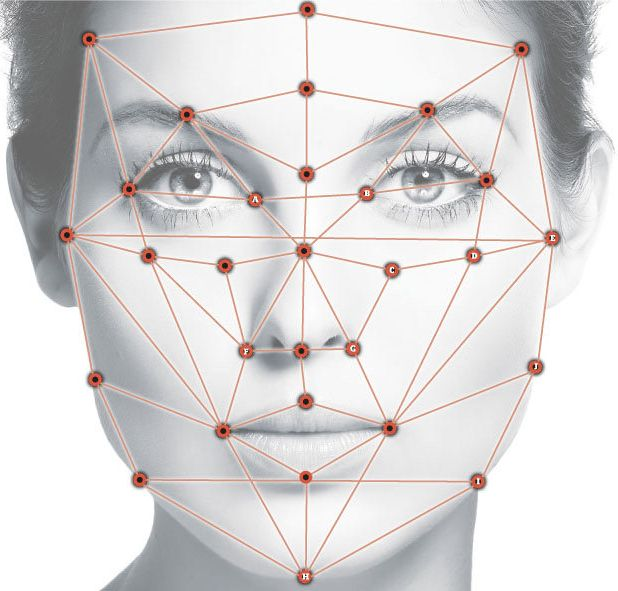
\includegraphics[scale=0.3]{face_map.jpg}}
\caption{Punkty charakterystyczne na twarzy człowieka}
\end{figure}

\end{frame}

%==============================
\begin{frame}
  \frametitle{Metody geometryczne}
 
Zalety:
\begin{itemize}
\item szybkość działania
\item zadowalające rezultaty działania
\end{itemize}

\vspace{10pt}
\uncover <2-> {
Wady:
\begin{itemize}
\item potrzeba precyzyjnego zlokalizowania odpowiednich fragmentów twarzy
\item zawodność metody gdy zdjęcie twarzy jest wykonane z profilu lub gdy część twarzy jest przysłonięta
\end{itemize}}

\vspace{10pt}
\uncover <3-> {
Obecnie, podejście to praktycznie nie jest już rozwijane, gdyż istnieją mechanizmy wykrywające twarze szybciej oraz z większą skutecznością.}

\end{frame}

%=============================================================
\subsection{Metoda analizy kolorów}
\begin{frame}
  \frametitle{Metoda analizy kolorów}

W metodzie tej na podstawie odpowiednich schematów kolorów wykrywa się wszystkie elementy na obrazie zgodne z danym schematem. W celu zlokalizowania twarzy należy dodatkowo przeprowadzić po niej selekcję po kształcie i rozmiarze wykrytych regionów.

\begin{figure}
 \only<1> {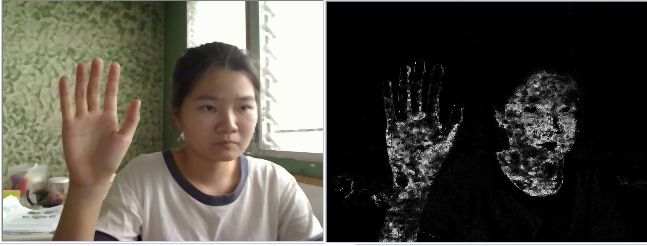
\includegraphics[scale=0.4]{skin_detection.jpg}}
\caption{Wykrywanie obszarów o kolorze skóry}
\end{figure}

\end{frame}

%==============================
\begin{frame}
  \frametitle{Metoda analizy kolorów}

Zalety:
\begin{itemize}
	\item szybkość działania
	\item brak ograniczeń odnośnie orientacji oraz rozmiaru twarzy
\end{itemize}

\vspace{10pt}
\uncover <2-> {
Wady:
\begin{itemize}
\item baza schematów kolorów jest ograniczona
\item duża podatność metody na natężenie jasności zdjęcia
\item obiekty o kolorze podobnym do koloru skóry są także wykrywane (np. ręce, szyja)
\end{itemize}
}

\end{frame}

%=============================================================
\subsection{Metoda sieci neuronowych}
\begin{frame}
  \frametitle{Metoda sieci neuronowych}

\begin{itemize}
\item Jedna z najczęściej używanych metod rozpoznawania twarzy
\item Odwzorowuje sposób działania neuronów w ludzkim mózgu
\item Przyjmuje na wejście wektor cech opisujący zlokalizowany obiekt, bądź cały obraz (CNN)
\item Zwraca na wyjście konkretną odpowiedź, w zależności od stanu wyuczenia sieci\\ (czy na obrazie jest twarz, czy też nie)
\end{itemize}

\end{frame}

%==============================
\begin{frame}
  \frametitle{Metoda sieci neuronowych}

Operację wykrywania twarzy za pomocą tej metody dzielimy na 3 etapy:
\begin{itemize}
\item Inicjalizacja\\ (projektowanie i tworzenie sieci neuronowych)
\item Trening\\ (wybór danych do trenowania, wybór cech, trenowanie)
\item Klasyfikacja\\ (skanowanie obrazów w celu zlokalizowania twarzy)
\end{itemize}

\end{frame}

%==============================
\begin{frame}
  \frametitle{Konwolucyjne sieci neuronowe (CNN)}

\uncover <1-> {
Konwolucyjne sieci neuronowe (CNN) pozwalają ominąć proces obróbki obrazu i ekstrakcji cech, kosztem trudniejszego etapu uczenia sieci.\\[\baselineskip]
}
\uncover <2-> {
Sieć uczona jest małymi obrazkami z samymi twarzami, a parametry sieci regulowane są za pomocą metody wstecznej propagacji.\\[\baselineskip]
}
\uncover <3-> {
W celu lokalizacji twarzy na wejście podawany jest cały obraz, a na wyjściu zmniejszony obraz punktów w których znajdują się twarze.\\[\baselineskip]
}
\uncover <4-> {
Po odpowiednim przeskalowaniu wyjścia otrzymujemy dokładną mapę lokalizacji i rozmiarów twarzy.
}
\end{frame}

%==============================
\begin{frame}
  \frametitle{Konwolucyjne sieci neuronowe (CNN)}

	\begin{figure}
    		\only<1> {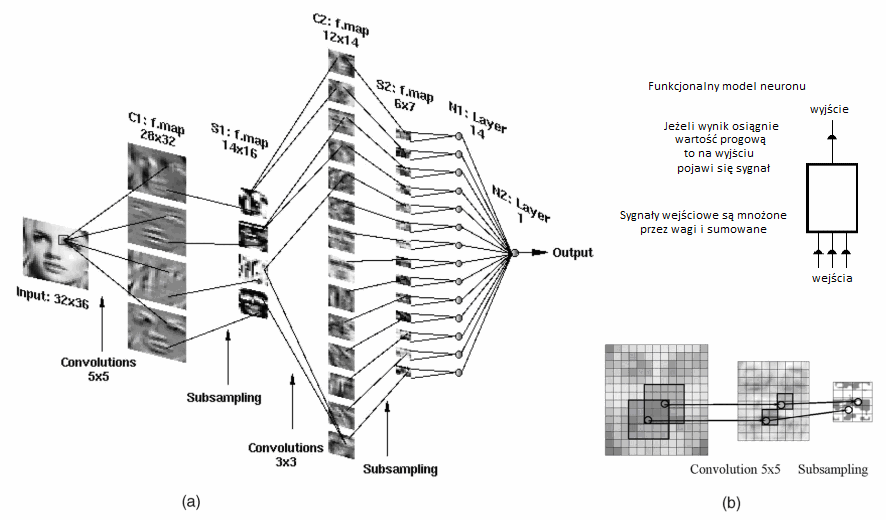
\includegraphics[scale=0.4]{cnn.png}}
		\caption{a) przykład konwolucyjnej sieci neuronowej (CNN) b) Operacja konwolucji i subsamplingu}
	\end{figure}

\end{frame}

%==============================
\begin{frame}
  \frametitle{Metoda sieci neuronowych}

\uncover <1-> { 
	Zalety:
	\begin{itemize}
		\item Bardzo dobre rozpoznawanie wzorców
		\item Praca z zaszumianymi i niepełnymi danymi
		\item Możliwość pracy równoległa z wielu wejść
		\item Rozwiązanie problemu bez jego dogłębnej analizy
		\item Duża tolerancja na błędy
	\end{itemize}
}

\vspace{10pt}
\uncover <2-> {
	Wady:
	\begin{itemize}
	\item  Długi czas uczenia
	\item Sukces uczenia nie jest gwarantowany
	\item Problemy z wyborem danych do treningu sieci
	\end{itemize}
}
\end{frame}

%=============================================================
\subsection{Model aktywnego kształtu}
\begin{frame}
  \frametitle{Model aktywnego kształtu}
  \begin{itemize}
  \uncover <1-> {\item Idea opracowana w 1995 roku przez Tim Cootesa oraz Chrisa Taylora}
  \uncover <2-> {\item Model statyczny, który "próbuje" dopasować się do obiektu na obrazie}
  \uncover <3-> {\item Wzorzec określany przez rozkład punktów}
  \uncover <4-> {\item Proces uczenia polega na zaznaczeniu punktów twarzy na wielu zdjęciach testowych}
  \uncover <5-> {\item Otrzymane wektory normalizuje się, po czym na podstawie średniego kształtu, odchylenia od średniej i macierzy kowariancji wyznaczony zostaje model}
 \end{itemize}
\end{frame}

%==============================
\begin{frame}
  \frametitle{Model aktywnego kształtu - maska}
\begin{center}
  \begin{figure}
    \only<1> {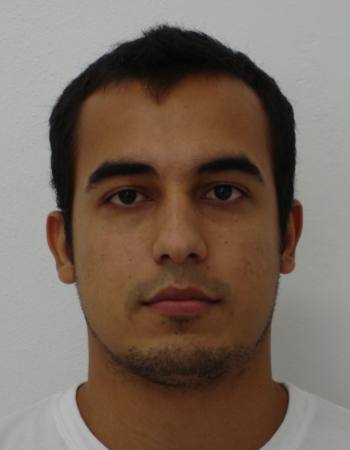
\includegraphics[scale=0.4]{aktywny2.png}}
    \only<2> {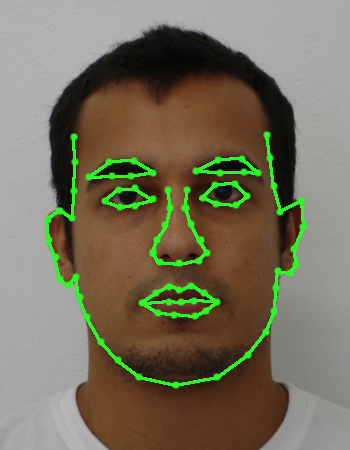
\includegraphics[scale=0.4]{aktywny3.png}}
    \only<3> {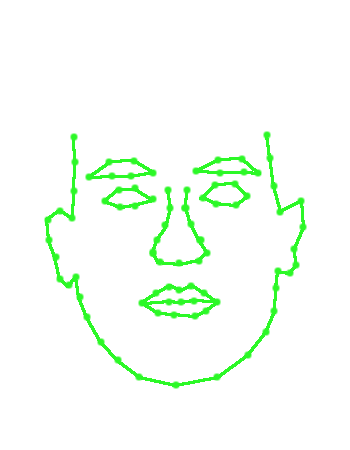
\includegraphics[scale=0.4]{aktywny1.png}}
    \caption{Przykład dopasowania maski}
  \end{figure}
\end{center}
\end{frame}

%==============================
\begin{frame}
  \frametitle{Model aktywnego kształtu \\ - lista kroków wyszukiwania obiektu}
  \begin{itemize}
\item Badane jest sąsiedztwo każdego punktu charakterystycznego w poszukiwaniu odpowiedniej deformacji
\item Obliczane są optymalne parametry przesunięcia, obrotu, skali tak aby umieścić niezdeformowany model jak najbliżej rzeczywistego kształtu
\item Uważając na dopuszczalny zakres zmian uaktualnia się parametry modelu dopasowując go jak najdokładniej do obrazu
\item Przesunięcie punktów charakterystycznych na podstawie krawędzi prostopadłych do brzegu modelu oraz poziomów jasności
\end{itemize}
\end{frame}

%==============================
\begin{frame}
  \frametitle{Model aktywnego kształtu - podsumowanie}
   \uncover <1-> { Zalety:
\begin{itemize}
\item Duża elastyczność - model potrafi dopasować się do różnych kształtów
\item Uniwersalny - kształt określany jest w drodze uczenia
\item Pomocny przy klasyfikowaniu i identyfikowaniu twarzy
\end{itemize}
}
  \uncover <2-> {\noindent 
Wady:
\begin{itemize}
\item  Czasochłonne i trudne uczenie modelu 
\item  Mało odporny na zmieniające się warunki oświetlenia, zróżnicowanego tła, bardziej realistycznych warunków
\item  Słabe wyniki dla osób z długimi ciemnymi włosami
\end{itemize}}
\end{frame}

%=============================================================
\section{Porównianie}

\begin{frame}
  \frametitle{Porównanie}

  porównanie

\end{frame}

%=============================================================
\section{Podsumowanie}

\begin{frame}
  \frametitle{Podsumowanie}

  parę słów podsumowania tutaj

\end{frame}

\end{document}
